\documentclass[11pt, t]{beamer}
\usepackage{amsmath}
\usepackage{setspace}
\usepackage{float} 
\usepackage{multido}
\usepackage{multirow}
\usepackage{array}
\usepackage{enumerate}
\usepackage{booktabs}
\usepackage{indentfirst} 
\usepackage[style=mla]{biblatex}
\usepackage{setspace}
\usepackage{subcaption}
\usepackage{hyperref}
\usepackage{textpos}

\makeatletter
\let\@@magyar@captionfix\relax
\makeatother

\definecolor{Turquoise3}{RGB}{0, 134, 139}
\renewcommand{\emph}[1]{{\color{Turquoise3}\textsl{#1}}}
\newcommand{\C}{\mathbb{C}} \newcommand{\F}{\mathbb{F}} \newcommand{\R}{\mathbb{R}} \newcommand{\Q}{\mathbb{Q}}
\newcommand{\N}{\mathbb{N}}
\newcommand{\myseries}[2]{$#1_1,#1_2,\dots,#1_#2$}
\newcommand{\nullspace}{~\\[15pt]}
\newcommand{\Remark}{\textbf{Remark: }}
\newcommand{\Question}{\textbf{Question: }}
\newcommand{\Extension}{\textbf{Extension: }}
\newcommand{\scp}[2]{\langle\,#1\,,\,#2\,\rangle} \newcommand{\scpp}{\langle\,\cdot\,,\,\cdot\,\rangle}


\usetheme{Madrid}
\setbeamertemplate{navigation symbols}{}

\addtobeamertemplate{frametitle}{}{
\begin{textblock*}{100mm}(0.85\textwidth,-1cm)

\includegraphics[height=1cm]{logo.png}
\end{textblock*}}

\definecolor{themecolor}{RGB}{25,25,112} 

\usecolortheme[named=themecolor]{structure}

\setbeamertemplate{items}[default]

\hypersetup{
    colorlinks=true,
    linkcolor=themecolor,
    filecolor=themecolor,      
    urlcolor=themecolor,
    citecolor=themecolor,
}

\title{VV285 Discussion Class II:\\Line Integrals in Mathematics and Physics}
\subtitle{A Comparison of Techniques, Conventions and Culture}
\institute[UM-SJTU JI]{Univerity of Michigan-Shanghai Jiao Tong University Joint Institute}
\author{Xingjian Zhang}

\begin{document}

\begin{frame}
    \titlepage
    \begin{center}
        
\includegraphics[height=2cm]{logo2.png}
    \end{center}
\end{frame}


\section{Mathematics vs. Physics}
\begin{frame}
    \frametitle{Outline}
    \begin{spacing}{1.5}
        \tableofcontents[currentsubsection,hideothersubsections,sectionstyle=hide]
    \end{spacing}
\end{frame}

\begin{frame}
    \frametitle{Something you need to pay attention to...}
    Think More and Be Interactive!
    \begin{itemize}
        \item Do think more about the question.
        \item The class is designed to be interactive.
        \item You are welcome to ask questions in a adequate manner.
        \item Please open your camera so that I can receive more feedbacks from you. (Makes our life easier!)
    \end{itemize}
\end{frame}

\subsection{Overview}
\begin{frame}[allowframebreaks]
    \frametitle{Overview}

    Trust me, you will reopen your VV285 lecture slides again and again in your future study, no matter what your major is! Here is a list of courses where you will find learning well in VV285 is so useful:
    \begin{enumerate}
        \item VV214 \& 417: Linear Algebra
        \item VV286: Honors Math IV
        \item VV556 \& 557: Methods of Applied Mathematics I\&II
        \item VP150/160 \& VP250/260: (Honors) Physics I\&II
        \item VP390: Modern Physics
        \item VE230 \& VE330: Electromagnetics I\&II
        \item VM211: Introduction to Solid Mechanics
        \item VM320 \& 520: Fluid Mechanics \& Advanced Fluid Mechanics
        \item \dots
    \end{enumerate}
    \newpage\footnotesize
    In today's lecture, we will see the similarity and difference between line integral in maths and physics, and interpret every questionable detail of a typical physic solution in rigorous mathematical way. A comparison of techniques, convention and culture of maths and phyiscs will be made. By the end of today's lecture, you will have a basic understanding of the maths foundation beneath a physical approach, and will see how different notations can change our way of thinking. It is a precious ability for you to connect different disciplines together and find the consistency in them!
    \begin{figure}[h]
        \centering
        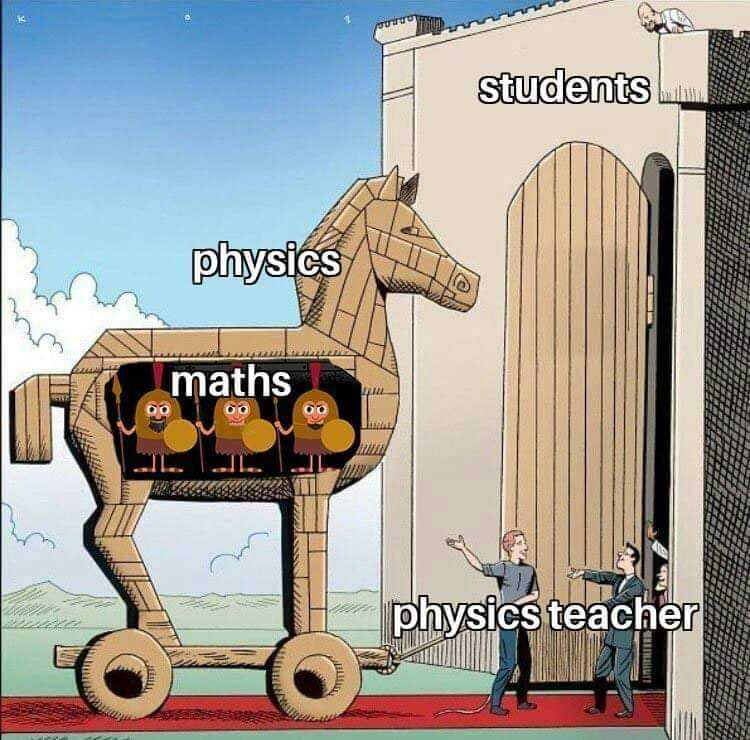
\includegraphics[width=0.35\textwidth]{2020-07-15-12-50-10.png}
    \end{figure}


\end{frame}

\subsection{Work}
\begin{frame}[allowframebreaks]
    \frametitle{Work}
    \begin{columns}
        \column{0.6\textwidth}
        Line integral (of vector field) has a very important physical application: the \emph{work}.\nullspace
        \textbf{Definition.} The work $W$ done by a constant force of magnitude $F$ on a point that moves a displacement $s$ in a straight line in the direction of the force is the product $$W=Fs.$$ We then generalize the concept of work to changing force and curving trajectory:
        $$W=\int_{\mathcal{C}^{*}} F d \vec{s}=\int_{\mathcal{C}^{*}}\langle F, d \vec{s}\rangle$$

        \column{0.3\textwidth}
        \begin{figure}[ht]
            \centering
            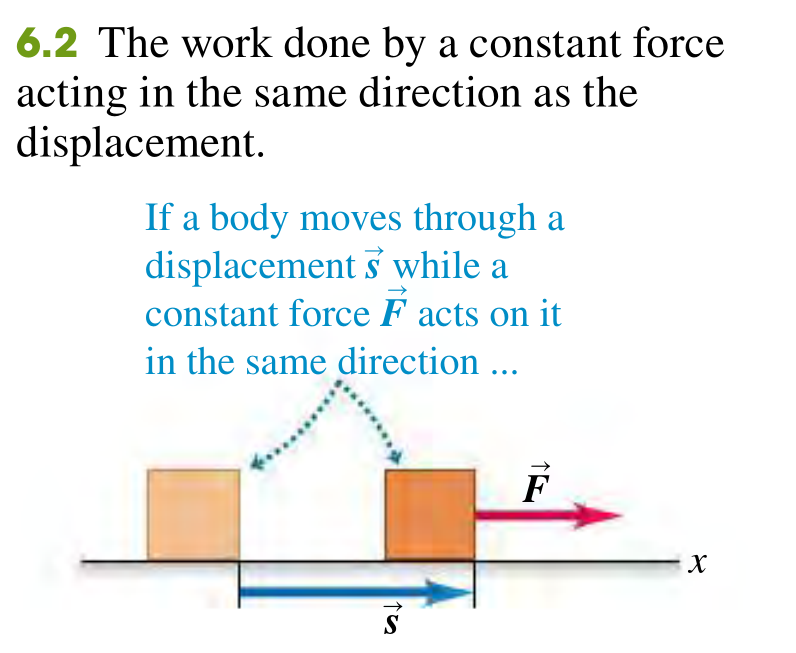
\includegraphics[width=\textwidth]{2020-07-15-10-14-01.png}
        \end{figure}
        \begin{figure}[ht]
            \centering
            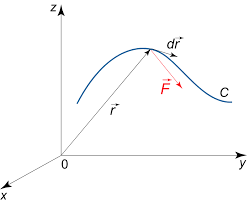
\includegraphics[width=\textwidth]{2020-07-14-22-23-32.png}
        \end{figure}
    \end{columns}
    \newpage
    Physicists always want a intuitive explanation of what's going on. Recall: how do we generalize the concept of work in VP160/VP150? We first establish a concept of \textit{elementary work}.\nullspace
    \textbf{Definition.} \emph{Elementary work} done by $F$ when the particle moves from $r$ to $r+d r$:
    \begin{equation}
        \qquad \delta W=\langle F,d r\rangle
        \vspace{10pt}
    \end{equation}
    We then define the work done by a force as the integration of all these elementary work. As a well-learned VV285 student, you probably find there are many issues in this definition. For example,
    \begin{itemize}
        \item we did not give a definition of $dr$, the so-called ``infinitesimal displacement''/``vectorial line element'',
        \item we assume $F$ does not change along this displacement,
        \item \dots
    \end{itemize}
    \newpage
    Though the definition of infinitesimal displacement $dr$ is not rigorous in the sense of mathematics, it is very intuitive and useful in simple situation. Later, we will see how this intuitive concept helps us solve some simple problems quickly.
    \begin{figure}[H]
        \centering
        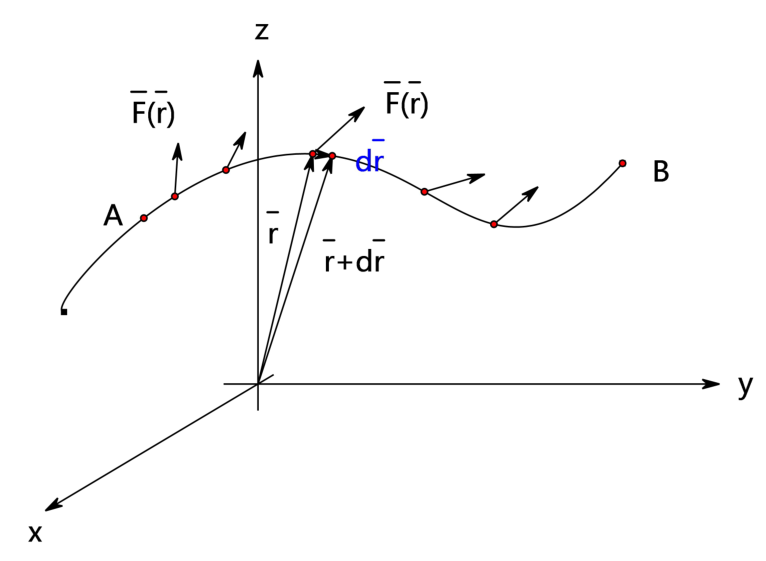
\includegraphics[width=0.4\textwidth]{2020-07-15-11-45-14.png}
        \caption{The Infinitesimal Displacement $dr$}
        \label{fig:}
    \end{figure}

    However, our intuitive method fails when things get a bit more complicated. We will also see some examples where an explicit parametrization is in need.
    \vspace{10pt}
    \begin{figure}[H]
        \centering
        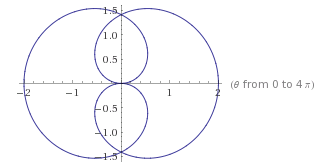
\includegraphics[width=0.4\textwidth]{2020-07-15-11-47-47.png}
        \caption{Complicated Situation where \\Elementary Physic Way Fails}
        \label{fig:}
    \end{figure}

\end{frame}

\subsection{Simple Examples}
\begin{frame}
    \frametitle{Example 1}
    Let's start with an simple example. Think twice about the difference between a mathematical approach and a typical physical approach. \nullspace
    \textbf{Problem.} Given a vector function $E=y\hat x+x\hat y$, evaluate the line integral $\int E\cdot d\ell$ from $P_1(2,1,-1)$ to $P_2(8,2,-1)$ along the parabola $x=2y^2$.\footnote[frame]{Problem 2-21 of VE230 Assignment 2 (2020 SU)}
    \begin{figure}[H]
        \centering
        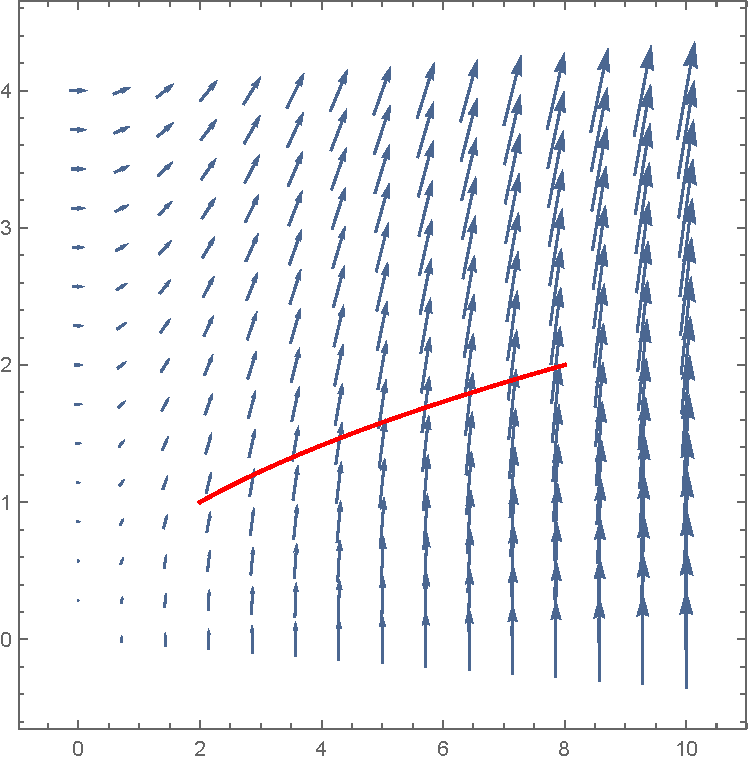
\includegraphics[width=0.3\textwidth]{e1.pdf}
        \label{fig:}
    \end{figure}
\end{frame}



\begin{frame}
    \frametitle{Example 1: Physic Approach}
    \textit{Below is a copy of solution to this question.}\footnote[frame]{VE230 TA's sample solution}\nullspace
    We want to solve $$\int_{P_1}^{P_2}E\cdot d\ell=\int_{P_1}^{P_2}(ydx+xdy).$$\\
    The trajectory is $x=2y^2$, so we have
    \begin{equation}\label{eq:subst}
        dx=4ydy.
    \end{equation}
    Insert this relation to our target integral, so we have $$\int_{1}^{2}(y(4ydy)+2y^2dy)=6\int_{1}^{2}y^2dy=14.$$
\end{frame}


\begin{frame}
    \frametitle{Example 2}
    Let's look at another example. We will use another method to solve this question.\\[8pt]
    Find the minimum work needed to move an object of weight $Q$, suspended on a light rod with length $R$, from $A$ to $B$, acting with a horizontal force.\footnote[frame]{VP160, s - 20hp09 - work and kinetic energy}
    \begin{figure}[H]
        \centering
        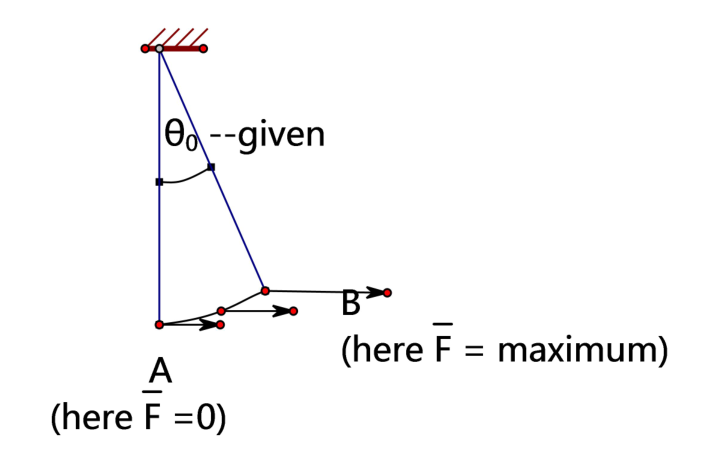
\includegraphics[width=0.6\textwidth]{2020-07-15-20-08-55.png}
    \end{figure}
\end{frame}

\begin{frame}[allowframebreaks]
    \frametitle{Example 2: Physic Approach}
    \textit{Below is a copy of solution to this question.}\footnote[frame]{VP160, s - 20hp09 - work and kinetic energy}\nullspace
    We decompose the elementary work
    $$\delta W=F \cdot d r=\left(F_{\|}+F_{\perp}\right) \cdot d r=\underbrace{F_{\|}}_{\text {varies}} \cdot d r$$ and express everything in terms of $\theta$. We find
    $$\delta W=F_\parallel|dr|=QR\sin\theta d\theta.$$
    \begin{figure}[H]
        \centering
        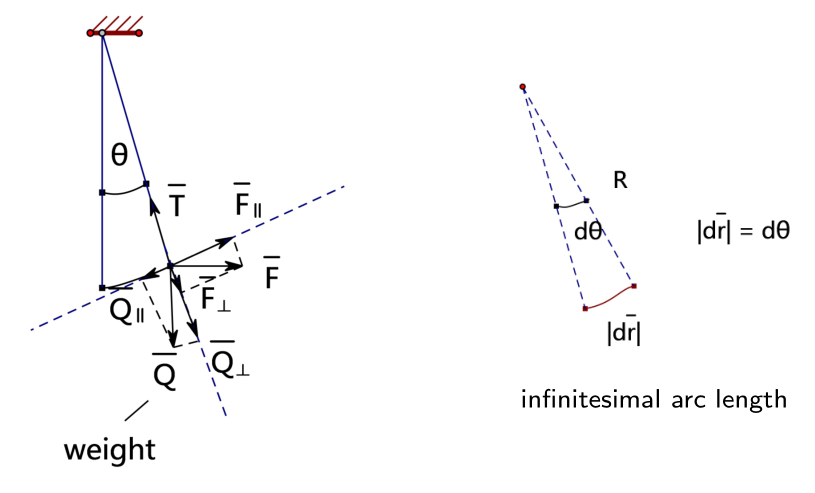
\includegraphics[width=0.5\textwidth]{2020-07-15-20-13-20.png}
    \end{figure}
    So the work done by $F$ on the path $A\to B$ (arc of a circle) is:
    $\begin{aligned}
            W_{A \rightarrow B} & =\int_{\Gamma_{A B}} F \cdot d r=\int_{0}^{\theta_{0}} \underbrace{Q \sin \theta}_{F_{\|}} R d \theta=Q R \int_{0}^{\theta_{0}} \sin \theta d \theta \\
                                & =Q R\left(1-\cos \theta_{0}\right)
        \end{aligned}$

\end{frame}

\begin{frame}
    \frametitle{Example 1: Mathematic Approach}
    \textit{Here is a math version of solution.}\nullspace
    As it indicates, the parametrization is $$\gamma:[1,2]\mapsto\mathcal{C},y\mapsto\begin{pmatrix}2y^2 \\      y\\
            -1
        \end{pmatrix}$$
    So we have $$E\circ\gamma(y)=\begin{pmatrix}
            y    \\
            2y^2 \\
            0
        \end{pmatrix},\qquad \gamma'(y)=\begin{pmatrix}
            4y \\
            1  \\
            0
        \end{pmatrix}$$
    We can then perform the integral:
    $$ \int_{1}^{2}\left\langle\begin{pmatrix}
            y    \\
            2y^2 \\
            0
        \end{pmatrix},\begin{pmatrix}
            4y \\
            1  \\
            0
        \end{pmatrix}\right\rangle dy=6\int_{1}^{2}y^2dy=14$$
\end{frame}

\begin{frame}
    \frametitle{Example 2: Mathematic Approach}
    \textit{Here is a math version of solution.}\nullspace
    We first write down the parametrization of the curve: $$\gamma:[0,\theta_0]\mapsto\mathcal{C},\theta\mapsto\begin{pmatrix}R\sin\theta \\ -R\cos\theta
        \end{pmatrix}$$
    So we have
    $$F\circ\gamma(\theta)=\begin{pmatrix}Q\tan\theta \\ 0
        \end{pmatrix},\qquad \gamma'(\theta)=\begin{pmatrix}R\cos\theta \\ R\sin\theta
        \end{pmatrix}$$
    We can then perform the integral:
    $$ \int_{0}^{\theta_0} \left\langle\begin{pmatrix}Q\tan\theta \\ 0
        \end{pmatrix},\begin{pmatrix}R\cos\theta \\ R\sin\theta
        \end{pmatrix}\right\rangle d\theta=QR\sin\theta d\theta=QR(1-\cos\theta_0).$$

\end{frame}

\subsection{A Comparison between Two Ways}
\begin{frame}
    \frametitle{A Comparison between Two Ways}
    Now you have seen the two different techniques. Can you find some differences or connections between them?\nullspace\pause
    After learning VV285, you are expected to know not only how to calculate but also \textbf{why we can do like that}. Let's go deeper into these question: Why the former method is feasible? What are we doing when we use a typical physical way?  Is there any limitations of this method?
\end{frame}

\subsection{Line Integral in Maths}
\begin{frame}
    \frametitle{Line Integral in Maths}
    Let $\Omega\subset\R^n,F:\Omega\to\R$ be a continuous vector field and $\mathcal{C}^*\subset\Omega$ on oriented open, smooth curve in $\R^n$. We then define the \emph{line integral of the vector field $F$ along $\mathcal{C}^*$} by
    \begin{equation}\label{3.1.5}
        \int_{\mathcal{C}^*}F\,d\vec{s}:=
        \int_{\mathcal{C}^*}\scp{F}{T}\,d\vec{s}
    \end{equation}

    \Remark \\In the rigorous maths version of line integral, we
    \begin{itemize}
        \item always have an explicit parametrization,
        \item utilize the tangent vector,
    \end{itemize}
    To calculate the line integral of a vector function, we
    \begin{enumerate}
        \item choose a suitable parametrization $\gamma:I\to\mathcal{C},t\mapsto\gamma(t)$,
        \item represent the vector function $F$ using $\gamma$, i.e. find $F\circ\gamma$
        \item find $\gamma\prime$
        \item perform integral $$\int_{I}\left\langle F \circ \gamma(t), \gamma^{\prime}(t)\right\rangle d t$$
    \end{enumerate}
\end{frame}

\subsection{Line Integral in Physics}
\begin{frame}[allowframebreaks]
    \frametitle{Line Integral in Physics}
    In physics, we approach to a question in term of infinitesimal displacement.
    \begin{figure}[H]
        \centering
        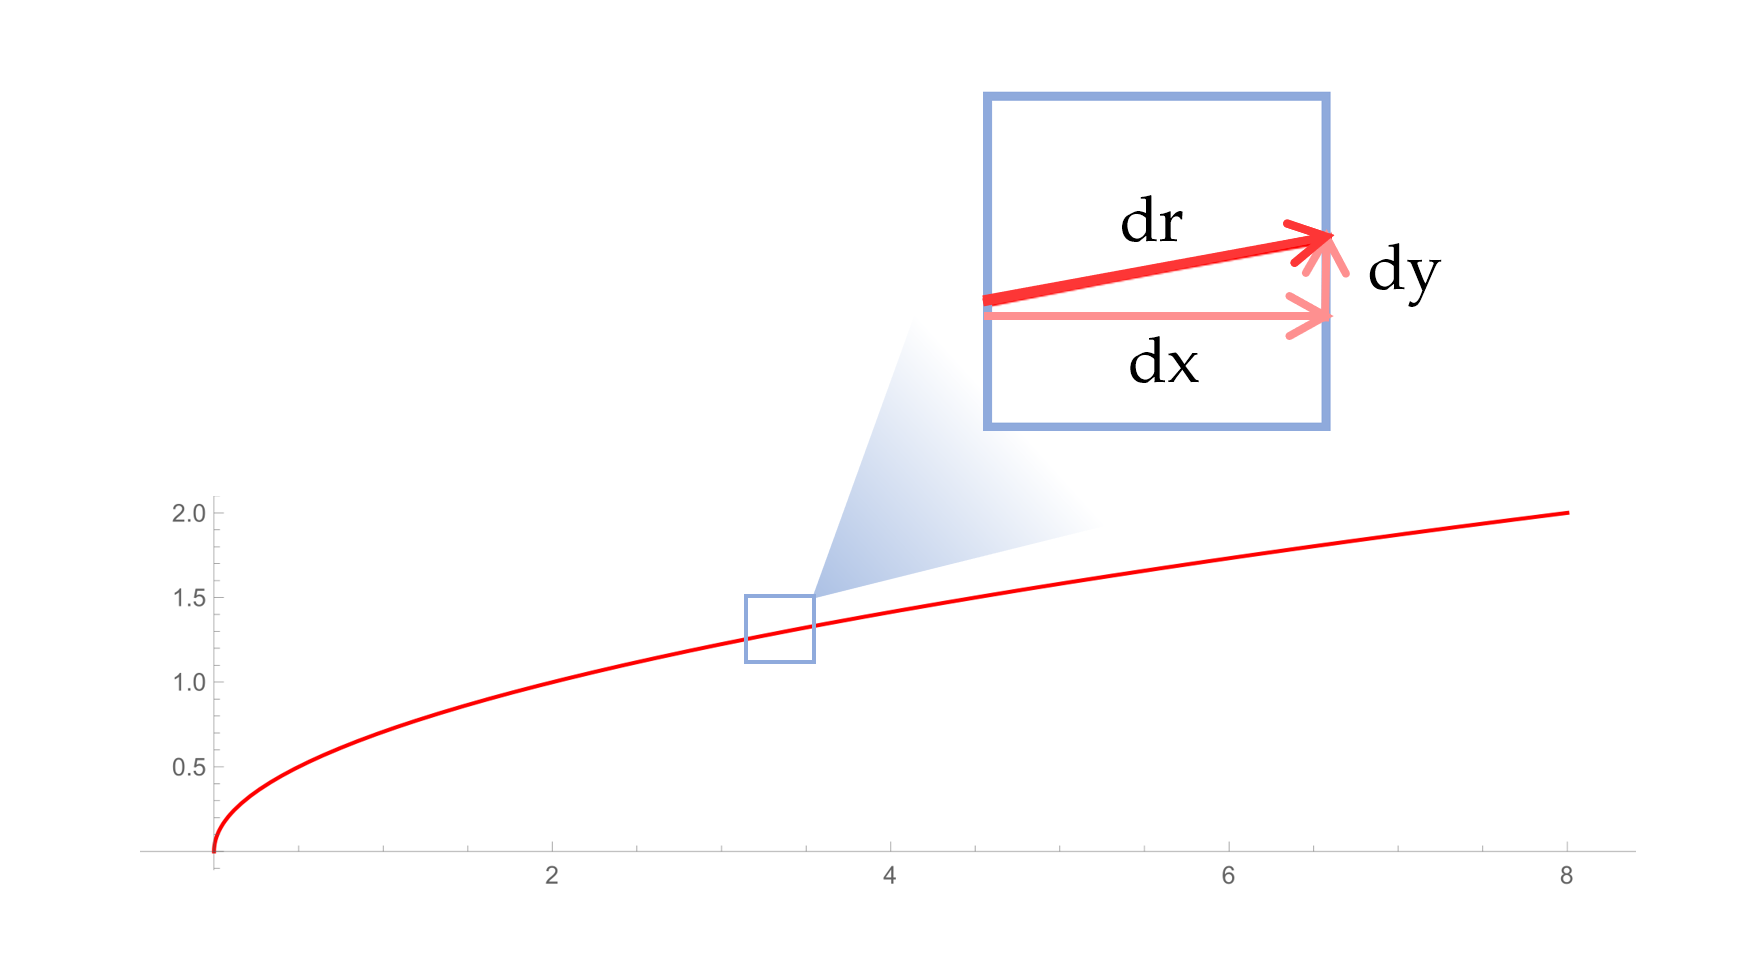
\includegraphics[width=0.4\textwidth]{2020-07-15-15-30-11.png}
        \caption{The relationship between $dx, dy$ and $dr$}
    \end{figure}
    Eq.\ref{eq:subst} is not strict in maths. It decomposes $dr$ into two orthogonal infinitesimal displacement $dx$ and $dy$. Then we get $\frac{dx}{dy}=4y$ through the derivative. Everything seems quite intuitive here, but it lacks a solid foundation. To some extent, it works because we adopted the \emph{Leibniz notation} here, which is extremely versatile and flexible.
    \newpage
    The physical approach might remind us the \emph{differential form} we learned in VV285.\nullspace
    \textbf{Definition. }Let $F_{1}, \ldots, F_{n}: \mathbb{R}^{n} \rightarrow \mathbb{R}$ be scalar functions. Then
    \[
        \alpha=F_{1} d x_{1}+\cdots+F_{n} d x_{n}
    \]
    is said to be a \emph{differential one-form}. We then simply define
    \[
        \int_{\mathcal{C}^{*}} \alpha:=\int_{\mathcal{C}^{*}} F d \vec{\ell}
    \]
    where $F=\left(F_{1}, \ldots, F_{n}\right)^{T}$ is the transpose of the differential form $\alpha$\nullspace
    \newpage
    However, they have totally different meanings! In physics, we consider $dx,dy$ and etc. as infinitesimal displacement with different ``lengths''. In mathematics (more precisely, differential geometry), we consider them as merely standard basis. So they certainly all have the unit length.
    \nullspace
    (Recall we define $x_j$ as $j^{th}$ coordinate map and $dx_j$ as the derivative of this map, which is equal to the $j^{th}$ standard basis row vectors.)
    \newpage
    Surprisingly, in practice we can solve the same problem in both two ways and always get the same answer! What's more, they looks totally the same because they adopt the same notation. The ambiguity of Leibniz notation turns out to be extremely convenient by this coincidence. Because the physic method is intuitive and the mathematic method is rigorous, they are complementary. The following example is solved using differential form, but we can interpret it perfectly using ``infinitesimal method''.\\[8pt]
    We integrate the form $4y\,dx+2x^2y\,dy$ in counter-clockwise direction along the unit circle $S^1\subset\R^2$. We parametrize the circle by $\gamma(\theta)=(\cos\theta,\sin\theta),0\leq
        \theta<2\pi$,\footnote[frame]{From VV285 course slide.}
    $$\begin{aligned}
            \oint_{S^{1}} 4 y d x+2 x^{2} y d y & =\oint_{S^{1}}\left(\begin{array}{c}
                    4 y \\
                    2 x^{2} y
                \end{array}\right) d \vec{\ell}                                                         \\
                                                & =\int_{0}^{2 \pi}\left(4 \sin \theta \cdot(-\sin \theta)+2 \cos ^{2} \theta \sin \theta \cdot(\cos \theta)\right) d \theta \\
                                                & =-8 \pi
        \end{aligned}$$
    \newpage
    We can also interpret the physic method using the linearity of integrals as well as inner product. i.e.
    $$\int(f+g)=\int f+\int g,\quad \int(\lambda f)=\lambda\int f.$$
    Consider integral in $\R^2$, we decompose it into 4 components:
    $$\int\left\langle\begin{pmatrix}
            F_x \\F_y
        \end{pmatrix},\begin{pmatrix}
            \gamma'_x \\\gamma'_y
        \end{pmatrix}\right\rangle dt=
        \int\left\langle\begin{pmatrix}
            F_x \\0
        \end{pmatrix},\begin{pmatrix}
            \gamma'_x \\0
        \end{pmatrix}\right\rangle dt+
        \int\left\langle\begin{pmatrix}
            F_x \\0
        \end{pmatrix},\begin{pmatrix}
            0 \\\gamma'_y
        \end{pmatrix}\right\rangle dt$$$$+
        \int\left\langle\begin{pmatrix}
            0 \\F_y
        \end{pmatrix},\begin{pmatrix}
            \gamma'_x \\0
        \end{pmatrix}\right\rangle dt+
        \int\left\langle\begin{pmatrix}
            0 \\F_y
        \end{pmatrix},\begin{pmatrix}
            0 \\\gamma'_y
        \end{pmatrix}\right\rangle dt$$
    $$=\int\left\langle\begin{pmatrix}
            F_x \\0
        \end{pmatrix},\begin{pmatrix}
            \gamma'_x \\0
        \end{pmatrix}\right\rangle dt+\int\left\langle\begin{pmatrix}
            0 \\F_y
        \end{pmatrix},\begin{pmatrix}
            0 \\\gamma'_y
        \end{pmatrix}\right\rangle dt$$
    $$=\int F_x dx+\int F_ydy$$
    \newpage
    In example 1, we happen to have $t=y$, so
    $$\gamma(t)=\gamma(y)=\begin{pmatrix}
            x \\y
        \end{pmatrix}=\begin{pmatrix}
            2y^2 \\y
        \end{pmatrix}$$

    Then we have $\gamma_x'=\frac{dx}{dy}=4y$. This also explains the meaning of Eq.\ref{eq:subst}.
    \newpage
    \Remark:\\
    In summary, in the physic way of line integral, we
    \begin{itemize}
        \item do not necessarily have a parametrization,
        \item consider infinitesimal displacement
        \item utilize the decomposition of force/displacement.
    \end{itemize}
    To calculate the line integral of a vector function, we
    \begin{enumerate}
        \item find the related infinitesimal displacement $dr$,
        \item decompose $F, dr$ into different directions, and represent them using a single variable, or
              \\ decompose the force $F$ into two components $F_\perp, F_\parallel$, and regard it as a line integral of scalar function,
        \item perform integral $\int F_xdx+F_ydy+F_zdz$ or $\int F_\parallel dr$.
    \end{enumerate}
\end{frame}



\subsection{Complicated Examples}
\begin{frame}
    \frametitle{Example 3}
    Let's see some complicated examples. We cannot solve them easily by the physic method without recourse to a parametrization.\nullspace
    A particle $p$ moves in a force field $F(x,y)=(-xy,x)$ along with the below trajectory. Calculate the work done by this force. Is it feasible to use a typical physic approach in this case?
    \begin{columns}
        \column{0.5\textwidth}
        \begin{figure}[H]
            \centering
            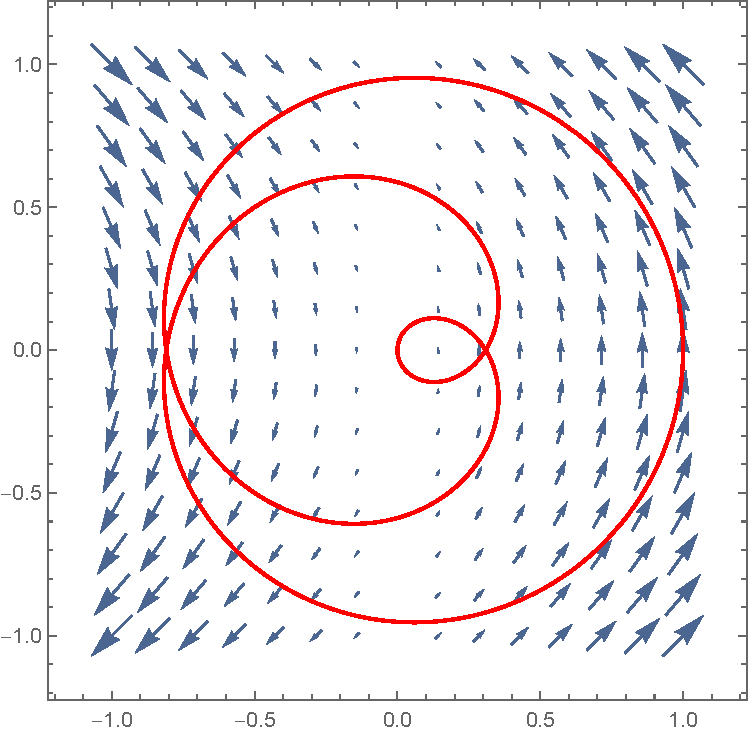
\includegraphics[width=0.7\textwidth]{c1.pdf}
        \end{figure}
        \column{0.5\textwidth}
        \vspace{1.5cm}

        $r=\cos(\dfrac{\theta}{5})$, $\theta\in[0,5\pi]$\\ \small The particle starts moving counter-clockwise.
    \end{columns}
\end{frame}

\begin{frame}
    \frametitle{Example 3: An Attempt Using Physic Approach}
    We first try to use the ``infinitesimal method''. We find a infinitesimal displacement, and decompose it into two orthogonal components.  \nullspace
    \begin{itemize}
        \item[$dxdy$] We find it hard to represent one using the other because the map is not injective. Thus, we cannot  find a way to perform integral.
        \item[$drd\theta$] We find it hard to decompose the force field onto the corresponding directions. (It is still possible to do so, but it takes extra effort to figure out the geometrical relationship.)
        \item[$F_\parallel F_\perp$] Similarly, we find it hard to find the geometrical relationship (In fact, we need extra effort to find them).
    \end{itemize}
    \nullspace
    In this situation, we find the physic method no longer convenient. And let's retry in a systematic math way.
\end{frame}

\begin{frame}
    \frametitle{Example 3: Mathematic Approach}
    Our parametrization is
    $$\gamma:[0,5\pi]\to \mathcal{C},\theta\mapsto\begin{pmatrix}
            \cos\frac{\theta}{5}\cos\theta \\
            \cos\frac{\theta}{5}\sin\theta
        \end{pmatrix}.$$
    Then, we have
    $$F\circ\gamma(\theta)=\begin{pmatrix}
            \cos^2\frac{\theta}{5}\cos\theta\sin\theta \\
            \cos\frac{\theta}{5}\cos\theta
        \end{pmatrix},\qquad \gamma'(\theta)=\begin{pmatrix}
            -\frac{1}{5}\cos\theta\sin\frac{\theta}{5}-\cos\frac{\theta}{5}\sin\theta \\
            -\frac{1}{5}\sin\theta\sin\frac{\theta}{5}+\cos\frac{\theta}{5}\cos\theta
        \end{pmatrix}$$
    Perform the integral,
    $$W=\int_0^{5\pi}\left\langle\begin{pmatrix}
            \cos^2\frac{\theta}{5}\cos\theta\sin\theta \\
            \cos\frac{\theta}{5}\cos\theta
        \end{pmatrix},\begin{pmatrix}
            -\frac{1}{5}\cos\theta\sin\frac{\theta}{5}-\cos\frac{\theta}{5}\sin\theta \\
            -\frac{1}{5}\sin\theta\sin\frac{\theta}{5}+\cos\frac{\theta}{5}\cos\theta
        \end{pmatrix}\right\rangle d\theta=\dfrac{5\pi}{4}.$$

\end{frame}

\begin{frame}
    \frametitle{Example 4}
    Here is an example that it is nearly impossible to be solved by a physic approach. The curve below is called a \textit{Folium of Descartes}. A particle moves along with this curve from $t=0.1$ to $t=10$ (in red) under the force field $F(x,y)=(\dfrac{3y^2}{x^4},\dfrac{3y^2}{x^4})$. Calculate the work done by $F$.
    \begin{columns}
        \column{0.5\textwidth}
        \begin{figure}[H]
            \centering
            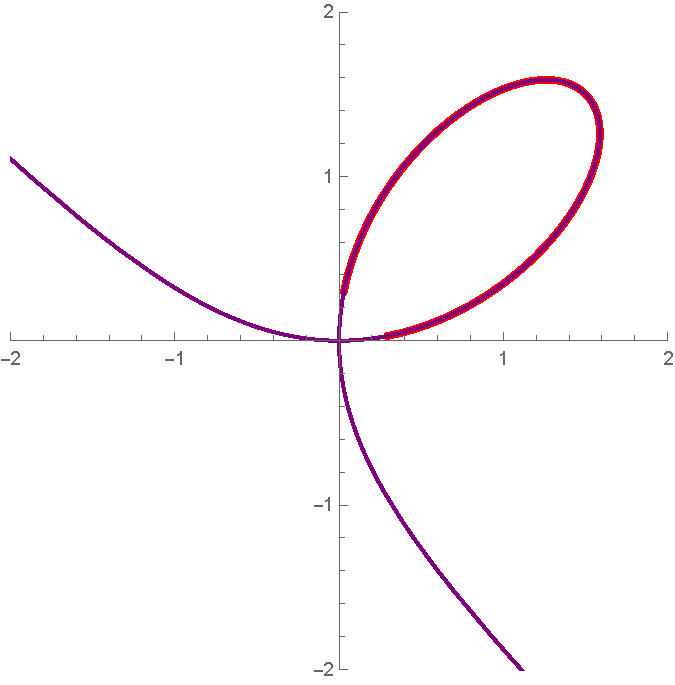
\includegraphics[width=0.7\textwidth]{c2.pdf}
        \end{figure}
        \column{0.5\textwidth}
        \vspace{1.5cm}

        $\gamma(t)=(\dfrac{3t}{1+t^3},\dfrac{3t^2}{1+t^3})$, $t\in\R.$\footnote[frame]{The curve can also be represented by a implicit function: $ x^3 + y^3 = 3xy.$}\\
    \end{columns}

\end{frame}

\begin{frame}
    \frametitle{Example 4: An Attempt Using Physic Approach}
    Let's still try to use the ``infinitesimal method'' to find the solution. However,  \nullspace
    \begin{itemize}
        \item[$dxdy$] We find it hard to represent one using the other because the map is not injective. Thus, we cannot find a way to perform integral.
        \item[$drd\theta$] We do not have a polar expression. So we cannot use this way.
        \item[$F_\parallel F_\perp$] We find it really hard to find the geometrical relationship. (At least we need tedious analysis to get one.)
    \end{itemize}
    \nullspace
    In this situation, the physic approach completely fails. So let's retry in a systematic math way.
\end{frame}

\begin{frame}
    \frametitle{Example 4: Mathematic Approach}
    We use the given parametrization
    $$\gamma:[0.1,10]\to\mathcal{C},t\mapsto\begin{pmatrix}
            \frac{3t}{1+t^3} \\\frac{3t^2}{1+t^3}
        \end{pmatrix}.$$
    And we have
    $$F\circ\gamma(t)=\begin{pmatrix}
            \frac{(1+t^3)^2}{3} \\
            \frac{(1+t^3)^2}{3}
        \end{pmatrix},\qquad
        \gamma'(t)=\begin{pmatrix}
            -\frac{9t^3}{(1+t^3)^2}+\frac{3}{1+t^3} \\
            -\frac{9t^4}{(1+t^3)^2}+\frac{6t}{1+t^3}
        \end{pmatrix}
    $$
    Then, we can perform the integral
    $$
        W=\int_{0.1}^{10}\left\langle \begin{pmatrix}
            \frac{(1+t^3)^2}{3} \\
            \frac{(1+t^3)^2}{3}
        \end{pmatrix},\begin{pmatrix}
            -\frac{9t^3}{(1+t^3)^2}+\frac{3}{1+t^3} \\
            -\frac{9t^4}{(1+t^3)^2}+\frac{6t}{1+t^3}
        \end{pmatrix}\right\rangle dt$$ $$=\int_{0.1}^{10}1 + 2 t - 2 t^3 - t^4dt=-24890.1$$
\end{frame}

\subsection{A Comparison between Notations}
\begin{frame}
    \frametitle{A Comparison between Notations}
    At this moment, we have compared the the two techniques in details. Just as the differences in techniques, we may also see different notations of vector calculus in various courses. Generally speaking, physicists prefer to use ``nabla'' ($\nabla$) and mathematicians prefer to use words.\footnote[frame]{Feynman Lectures, Chapter 11, Vol. I, Vectors}
    \begin{table}[htbp]
        \centering
        \caption{A Comparison of two Types of Notations}
        \begin{tabular}{cc}
            \hline
            Physics          & Mathematics             \\ \hline
            $\nabla U$       & $\operatorname{grad} U$ \\
            $\nabla\cdot F$  & $\operatorname{div} F$  \\
            $\nabla\times F$ & $\operatorname{curl} F$ \\
            $\nabla^2 U$     & $\Delta U$              \\ \hline
        \end{tabular}
    \end{table}

\end{frame}
\subsection{A Comparison between Culture}
\begin{frame}[allowframebreaks]
    \frametitle{A Comparison between Culture}
    The divergence between physicists and mathematicians is large in term of ``culture''. While mathematicians pursue precision, strictness, and logic, physicist pursue a sense of intuition. Let's read the comments made by Richard Feynman:
    \begin{quote}
        It will take you some time to understand what should happen in different circumstances. You will have to solve the equations. Each time you solve the equations, you will learn something about the character of the solutions. To keep these solutions in mind, it will be useful also to study their meaning in terms of field lines and of other concepts. This is the way you will really “understand” the equations. That is the difference between mathematics and physics.
    \end{quote}
    \begin{quote}
        Mathematicians, or people who have very mathematical minds, are often led astray when “studying” physics because they lose sight of the physics. They say: “Look, these differential equations—the Maxwell equations—are all there is to electrodynamics; it is admitted by the physicists that there is nothing which is not contained in the equations. The equations are complicated, but after all they are only mathematical equations and if I understand them mathematically inside out, I will understand the physics inside out.” Only it doesn’t work that way. Mathematicians who study physics with that point of view—and there have been many of them—usually make little contribution to physics and, in fact, little to mathematics. They fail because the actual physical situations in the real world are so complicated that it is necessary to have a much broader understanding of the equations.
    \end{quote}
    \begin{quote}
        What it means really to understand an equation—that is, in more than a strictly mathematical sense—was described by Dirac. He said: “I understand what an equation means if I have a way of figuring out the characteristics of its solution without actually solving it.” So if we have a way of knowing what should happen in given circumstances without actually solving the equations, then we “understand” the equations, as applied to these circumstances. \textbf{A physical understanding is a completely unmathematical, imprecise, and inexact thing, but absolutely necessary for a physicist}.\footnote[frame]{Feynman Lectures, Chapter 11, Vol. I, Vectors}
    \end{quote}
    
    \newpage
    To some extent, the comments made by Feynman explains why physicists love techniques like ``infinitesimal method'' or notations like Leibniz notations: They are extremely user-friendly and intuitive, making sense to any person who does not necessarily know the strict math foundations. \nullspace
    If you want to find more materials about the cultural difference between mathematicians and physicists. Here is a link for your reference:
    \href{https://medium.com/cantors-paradise/richard-feynman-on-the-differences-between-mathematics-and-physics-c0847e8a3d75}{Richard Feynman on the Differences between Mathematics and Physics}.
    \nullspace
    Another interesting study on physicists: \href{https://phys.org/news/2016-11-physicists-mathematics.html}{Even physicists are 'afraid' of mathematics}
\end{frame}

\begin{frame}
    \frametitle{Summary}
    As a engineering student, to calculate complicated integral is a basic ability. However, it is more precious an ability to understand the principles beneath the application. Because you only learned techniques in the former case, but learned a way of thinking in the later one. In the future study, you will encounter more difficult problems (not only regarding maths). At that moment, you will expect yourself to know how everything is going on. \nullspace
    
    Mathematics is beautiful, but the real world is chaotic. Knowing how to apply the math into real engineering problems is an important skill. I hope what you learned today can help you establish a better understanding of integral, thus can better deal with the chaotic real world.
    \nullspace    

\end{frame}


\begin{frame}
    \frametitle{Discussion}
    \vspace{1cm}
    \begin{center}
        \LARGE
        Have Fun\\
        And\\
        Learn Well!
    \end{center}
\end{frame}

\end{document}